\chapter{Die Eclipse Plattform}
\label{chap:platform}

In diesem Kapitel wird gezeigt, was Eclipse für Möglichkeiten bietet, um eine moderne Entwicklungsumgebung zu implementieren. Die verschiedenen Möglichkeiten werden miteinander Verglichen und die Vor- und Nachteile aufgezeigt. Auch werden die wichtigsten Eclipse Features, welche für das Entwickeln von Eclipse Rich Client Platform (RCP) Applikationen benötigt werden, beschrieben.

\section{Eclipse Plattform}

Eclipse RCP bietet eine Basis um beliebige, nicht zwingendermassen Entwicklungsumgebungen, Betriebssystem unabhängige, Applikationen zu entwickeln. Es bietet Mechanismen, wie Plugins und Extension Points, um modulares programmieren zu unterstützen und vereinfachen. Auch bietet das Framework Features wie Views, Editoren und Perspektiven welche häufig in Applikationen gebraucht werden.

\section{Plugins}

Eclipse Applikationen nützen eine auf der OSGi Speizifikation basierten Runtime. Eine Komponente in dieser Runtime ist ein Plugin. Eine Eclipse RCP Applikation besteht aus einer Ansammlung dieser Plugins.\cite{whatisaplugin} Plugins haben einen Lebenszyklus und können zur Laufzeit geladen oder entladen werden. Ein Eclipse Plugin kann Extension Points anderer Plugins ansteuern und eigene Extension Points oder APIs anbieten.

\section{Extension Points}
\label{extensionpointssection}

Um Plugins erweitern zu können, bietet Eclipse das Konzept von Extension Points an. Über Extension Points können Plugins ein bestimmte Funktionalität anbieten, welche von anderen Plugins angesteuert werden kann. 
\newline
Eclipse bietet ein Plugin an, welches einen Extension Point für Views definiert. Andere Plugins können über diesen Extension Point, eine neue View erstellen und diese konfigurieren. \cite{extensionpoints}

\newpage
In der Abbildung \ref{fig:extensionpoint} ist zu sehen, wie über diesen Extension Point eine neue Eclipse View erstellt werden kann.
\begin{figure}[H]
	\centering
		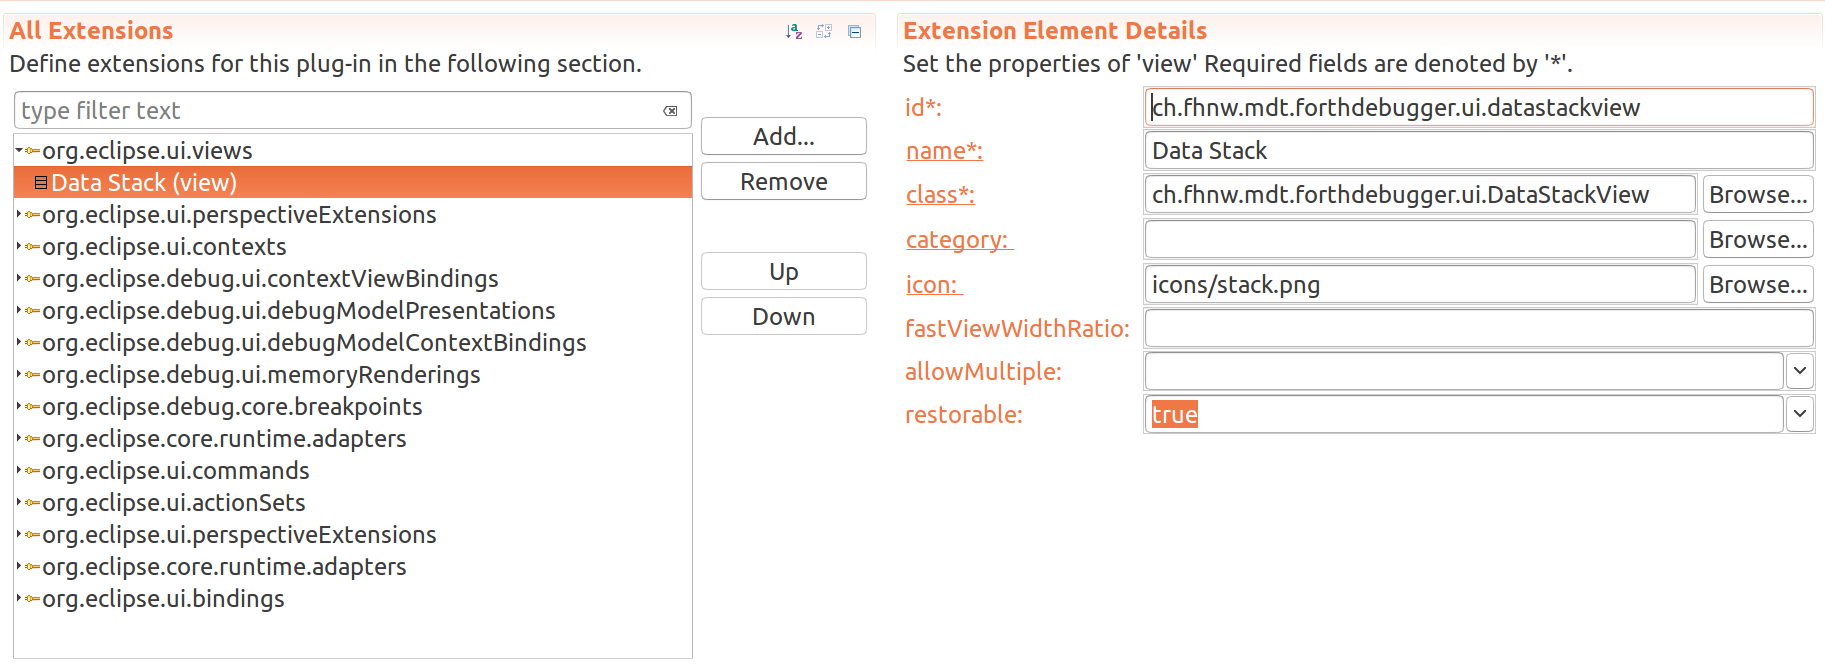
\includegraphics[scale=0.25]{platform/extensionpoint2.png}
		\caption{Ein Plugin, welches einen Extension Point anbietet. Andere Plugins können diese deklarativ in einem XML File ansteuern.}
		\captionsetup{margin=0cm,font={footnotesize}}
		\label{fig:extensionpoint}
\end{figure}

Es ist auch möglich eigene Extension Points zu definieren, falls ein Plugin für andere Entwickler offen stehen soll für Erweiterungen.

\section{Eclipse basierte MCore Entwicklungsumgebung}

Eclipse als Grundlage für eine Entwicklungsumgebung zu verwenden eignet sich besonders gut, da Eclipse schon einiges an Funktionalität für eine Entwicklungsumgebung zur Verfügung stellt und schon viele Entwicklungsumgebungen (PHP, C/C++, Pyhton und D unter anderem) basierend auf Eclipse entwickelt wurden. Auch existieren einige Tools, auf welche ich noch genauer eingehen werde, wie Xtext und DLTK, welche das entwickeln einer Entwicklungsumgebung weiter vereinfachen. In folgenden Kapiteln wird kurz auf die Möglichkeiten, welche von Eclipse bereitgestellten Technologien verwendet werden könnten um die Entwicklungsumgebung zu implementieren.

\subsection{JDT}
Eine Möglichkeit die MCore Entwicklungsumgebung zu implementieren wäre, die Standard Features von dem Eclipse Java Development Tools (JDT) zu verwenden. Dies wäre sehr Aufwendig, da alle Features für C, wie Syntax Highlighting, Code Completion oder eine Outline, neu implementiert werden müssten.

\subsection{Xtext}
XText ist ein Framework, welches es erleichtert, eine auf Eclipse basierte Entwicklungsumgebungen zu programmieren. Es ermöglicht auf schnelle Art und Weise das Grundgerüst einer Entwicklungsumgebung mit Features wie:

\begin{itemize} 
	\item Editor mit Syntax Coloring
	\item Code Completion
	\item Compiler Integration
	\item Java-basierter Debugger
	\item Outline
	\item Indexing
\end{itemize}

zu generieren. \cite{xtext} Es muss lediglich eine ANTLR\cite{antlr} ähnliche Grammatik für die Sprache definiert werden. Für den C-Editor eine Grammatik zu definieren ist schwierig, da dazu auch noch der Präprozessor mit einbezogen werden müsste. Für den Forth Editor kann Xtext verwendet werden. Im Kapitel \nameref{chap:fortheditor} wird beschrieben, wie Xtext verwendet wurde um einen Forth Editor zu implementieren.

\subsection{Dynamic Language Toolkit Framework}
Das Dynamic Language Toolkit (DLTK) ist ein weiteres Framework, welches das Grundgerüst für eine Entwicklungsumgebung generieren kann. Ursprünglicherweise war das Framework nur für dynamische Sprachen geeignet, es kann aber auch für statische Sprachen verwendet werden. Die D Entwicklungsumgebung wurde mit dem DLTK realisiert\cite{ddt}. Es bestehen aber wieder dieselben Nachteile wie bei Xtext. Da C schwierig zu parsen ist, müsste trotz dem Framework noch viel selbst implementiert werden. Die Sprache D verwendet keinen Präprozessor, deshalb konnte für diese Entwicklungsumgebung das DLTK Framework verwendet werden.

\subsection{Eclipse C/C++ Development Tools}
Das Eclipse C/C++ Development Tools (CDT), ist eine Eclipse Distribution mit Unterstützung für C und C++. Das CDT bietet viele Features, welche schon vom JDT bekannt sind, für C an und stellt Extension Points zur Verfügung um diese zu verwenden. So kann mit relativ wenig Aufwand einen neuen Compiler in die Entwicklungsumgebung eingebunden werden. Dies wurde auch schon mehrfach gebraucht, um verschiedene C/C++ Compiler im Eclipse CDT zu integrieren. Auf die Einbindung des Compilers wird im Kapitel \ref{compilerintegration} genauer eingegangen.

\subsection{Verwendung für uCore Eclipse}
Ich habe mich dazu entschieden, das Eclipse CDT als Target Platform zu wählen. Somit können alle Features, welche das Eclipse CDT zur Verfügung stellt, für die C Entwicklung gebraucht werden. Xtext kann zusätzlich noch verwendet werden, um den Forth Editor zu implementieren.
